\documentclass[aspectratio=169]{beamer}
\usetheme{Madrid}
\usecolortheme{seahorse}
\usefonttheme{professionalfonts}
\usepackage{amsmath,booktabs,tikz}
\usetikzlibrary{arrows.meta}
\setbeamertemplate{navigation symbols}{}
\renewcommand{\appendixname}{\texorpdfstring{\translate{Appendix}}{Appendix}}
\title[Policy evaluation]{Evaluating a Training Policy}
\author{Research Group}
\institute{Department of Economics}
\date{Research Seminar}
\AtBeginSection[]{\begin{frame}{Road map}\tableofcontents[currentsection]\end{frame}}
\begin{document}
\begin{frame}\titlepage\end{frame}
\begin{frame}{Outline}\tableofcontents\end{frame}
\section{Question and design}
\begin{frame}{Research question}
\begin{block}{Question}Does training raise participants' earnings?\end{block}
\begin{itemize}
\item<1-> Compare eligible and ineligible workers.
\item<2-> Observe earnings before and after implementation.
\item<3-> Check the plausibility of parallel trends.
\end{itemize}
\note{Distinguish the policy effect from selection into training.}
\end{frame}
\begin{frame}{Identification}
\begin{equation}
Y_{it}=\alpha_i+\lambda_t+\beta(D_i\times Post_t)+\varepsilon_{it}.
\label{eq:did}
\end{equation}
For an applied discussion, see \cite{angrist}.
\begin{alertblock}{Assumption}In the absence of treatment, groups would have parallel trends.\end{alertblock}
\end{frame}
\begin{frame}{Design in one picture}
\begin{columns}[T,onlytextwidth]
\begin{column}{.54\textwidth}
\centering
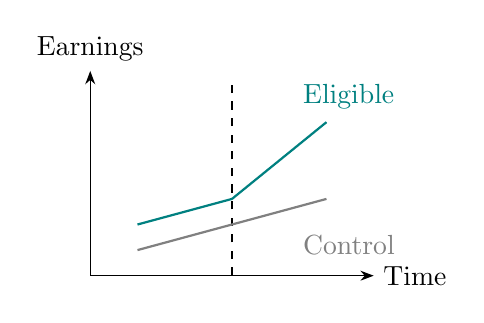
\begin{tikzpicture}[x=.6cm,y=.65cm,>=Stealth]
\draw[->] (0,0)--(6,0) node[right]{Time};
\draw[->] (0,0)--(0,4) node[above]{Earnings};
\draw[dashed] (3,0)--(3,3.8);
\draw[teal,thick] (1,1)--(3,1.5)--(5,3);
\draw[gray,thick] (1,.5)--(3,1)--(5,1.5);
\node[teal,right] at (4.3,3.5){Eligible};
\node[gray,right] at (4.3,.6){Control};
\end{tikzpicture}
\end{column}
\begin{column}{.42\textwidth}
The dashed line marks implementation. The drawing is schematic and contains no empirical observations.
\end{column}
\end{columns}
\end{frame}
\section{Results}
\begin{frame}{Illustrative estimates}
\centering
\begin{table}
\caption{Demonstration results, not research findings}
\begin{tabular}{lrr}
\toprule & Baseline & Controls \\
\midrule Training effect & 0.12 & 0.10 \\
Standard error & 0.04 & 0.03 \\
Observations & 800 & 800 \\
\bottomrule
\end{tabular}
\end{table}
\medskip
\uncover<2->{Report standard errors, units, sample restrictions, and the estimation method.}
\end{frame}
\begin{frame}{Interpretation and limitations}
\begin{itemize}
\item An estimate is meaningful only with a credible design.
\item Test alternative windows and inspect pre-treatment trends.
\item State the population to which the result applies.
\end{itemize}
\end{frame}
\begin{frame}{References}
\begin{thebibliography}{9}
\bibitem{angrist} Angrist, J. D. and Pischke, J.-S. (2009).
\newblock \emph{Mostly Harmless Econometrics}. Princeton University Press.
\end{thebibliography}
\end{frame}
\begin{frame}{Takeaway}
Design, evidence, and interpretation should answer the same research question.
\end{frame}
\appendix
\begin{frame}{Backup: the contrast}
\[\widehat\beta=(\overline Y_{T,post}-\overline Y_{T,pre})-(\overline Y_{C,post}-\overline Y_{C,pre}).\]
\end{frame}
\end{document}
